\subsubsection{Modelo Timers}

Este modelo representa la funcionalidad de un sistema de eventos por tiempo, ya sea mediante temporizadores periódicos a intervalos concretos o mediante periodos concretos \cite{scheduling_sporadic_aperiodic_events}.

Contamos con los siguientes eventos de tipo:

\begin{itemize}

\item \textit{NowEvent}. Representa un evento para disparar en el mismo momento de su ejecución.
\item \textit{RepeatedEvent}. Representa un evento que disparará cada x unidades de tiempo.
\item \textit{ClockEvent}. Representa un evento que dispará cada x hora/minuto/segundo definidas.
\item \textit{CronEvent}. Representa un evento que dispará cada x unidades definidas en formato Unix CRON.

\end{itemize}

Estos eventos utilizan como tipo de dato los elementos definidos en \textit{TimeUnit} y \texit{TimeUnitValue} para así poder identificar sin ningún error la unidad de tiempo definida.

A continuación podemos visualizar la representación en formato \gls{ecore} en la figura \ref{fig:modelo_timers_ecore} y la representación como diagrama de clases en la figura anexa  \ref{fig:modelo_timers_classes} de este modelo de datos.


El modelo eventos representa la base de todos los componentes que posteriormente modelaremos. Podemos observar en la figura \ref{fig:modelo_timers_ecore} la representación de este modelo en formato \gls{ecore} tree, generado en el propio entorno \gls{emf}.

\begin{figure}
	\centering
    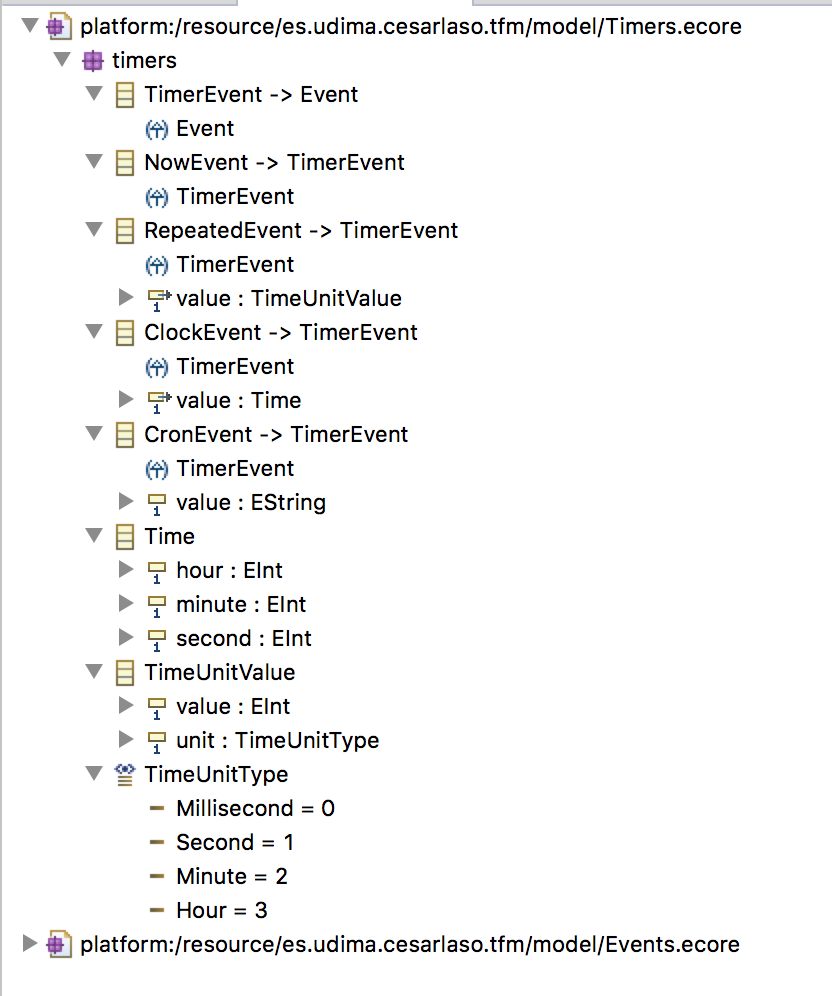
\includegraphics[scale=0.5]{images/emf_capturas/timers_ecore.png}
    \sourcepropia{}
    \captionmodelotree{Timers}
    \label{fig:modelo_timers_ecore}
\end{figure}
